\documentclass[aps,prl,twocolumn]{revtex4}
\usepackage{epsfig}
\usepackage{graphicx,psfrag,color}
\usepackage{bm}%bold math
\begin{document}


\title{Controlled-dipole quantum memory}

\author{Authors
%Yang Han$^{1,2}$, Khabat Heshami$^1$, Adam Green$^1$, Arnaud %Rispe$^1$, Erhan Saglamyurek$^1$, Neil Sinclair$^1$, Cheng-Zu Li$^2$, %Wolfgang Tittel$^1$, and Christoph Simon$^1$
}
\affiliation{$^1$ Institute for Quantum Information Science and
Department of Physics and Astronomy, University of Calgary,
Calgary T2N 1N4, Alberta, Canada\\
$^2$ National University of Defence Technology, Changsha, China}


\begin{abstract}
We present a quantum memory protocol for photons that is based on the direct control of the transition dipole moment. We focus on the case where the light-matter interaction is enhanced by a cavity. We show that the optimal write process is related to the optimal read process by a reversal of the {\it effective time} $\tau=\int dt g^2(t)/\kappa$, where $g(t)$ is the time-dependent coupling and $\kappa$ is the cavity decay rate. We discuss the implementation of the protocol in certain rare-earth doped crystals, where transitions can be turned on and off by switching a magnetic field.
\end{abstract}
\date{\today}

\maketitle

Quantum memories for light are devices that allow one to store and retrieve light in a way that preserves its quantum state \cite{lvovsky,hammerer,simonEPJD}. They are essential components for optical quantum information processing, notably for quantum repeaters \cite{sangouardRMP}. All quantum memories require a way of switching the coupling between the light and the material system (which is used as the memory) on and off in a controlled way. In the case of memories based on electromagnetically induced transparency or off-resonant Raman transitions \cite{lukinRMP,gorshkovPRL,EITexp,nunn,Ramanexp} the coupling is controlled by a laser beam, which is typically much more intense than the signal that one aims to store. In contrast, in the case of photon-echo based memories \cite{tittel,echoexp} the coupling is controlled in a more indirect way via the dephasing of the atoms in the storage medium. This typically requires spectral tailoring of the medium by optical pumping before the signal can be stored.

Here we consider a way of controlling the light-matter interaction that is different from the mentioned examples, and that is particularly simple from a conceptual point of view, namely the direct control of the transition dipole element of the relevant optical transition. This is motivated by recent demonstrations that transition dipoles can be turned on and off in certain solid-state systems, in particular in rare-earth doped crystals by applying magnetic fields \cite{Guillot-Noel,GenevaDipole}, and for NV centers in diamond by applying electric fields \cite{Tamarat}.
We consider the case where the storage medium is placed inside an optical cavity \cite{GorshkovCavity,IMQM,vuletic}. This both enhances the light-matter interaction, which is desirable for achieving high efficiencies, and simplifies the equations of motion, clearly bringing out the basic principles of the memory dynamics.

We consider an ensemble of two-level atoms coupled to a cavity mode, see also Fig. 1. We ignore the spatial dependence of the light-matter interaction, and thus phase-matching considerations \cite{kalachev}, which means that the equations below could also describe a single two-level system coupled to a cavity. We use the usual input-output formalism for a single-sided, fairly high-finesse cavity. The basic equations are then
\begin{eqnarray}
\dot{\sigma}(t)=-i \Delta(t) \sigma(t) - \gamma \sigma(t) + i g(t) E(t) \nonumber\\
\dot{E}(t)=ig(t) \sigma(t)-\kappa E(t) + \sqrt{2\kappa} E_{in}(t)\nonumber\\
E_{out}(t)=-E_{in}(t)+\sqrt{2\kappa} E(t).
\end{eqnarray}
Thanks to the linearity of the dynamics, $\sigma$ and $E$ can be interpreted as the atomic polarization and cavity fields (in the semi-classical regime), but also as the probability amplitudes corresponding to a single atomic excitation in the ensemble and a single cavity photon respectively (in the quantum regime, which is our focus here) \cite{hammerer,gorshkovPRL,GorshkovCavity}; $E_{in}$ and $E_{out}$ are the incoming and outgoing fields (photon wave functions); $g(t)$ is the time-dependent light-matter coupling, which is proportional to the transition dipole matrix element between the ground and excited atomic states (and also to $\sqrt{N}$, where $N$ is the total number of atoms); $\kappa$ is the cavity decay rate; $\gamma$ is the atomic decay rate; $\Delta(t)$ is a time-dependent detuning which may arise in practice as a consequence of applying a time-dependent external field in order to control the dipole element and thus $g(t)$; $\gamma$ and $\Delta(t)$ are imperfections which we will neglect at first to keep the discussion simple, but whose effect will be discussed later in the paper. The described system is equivalent to a Raman memory in a cavity, if the excited state is adiabatically eliminated in the Raman case \cite{GorshkovCavity}, and where the two-photon spin transition is replaced by a single-photon optical transition.


%\begin{figure}
%\epsfig{file=Figure1.eps,angle=270,width=0.6 \columnwidth}
%\caption{We consider an ensemble of two-level systems inside a one-sided cavity, where the time-dependence of the light-matter coupling $g(t)$ can be controlled. See also Eq. (1).} \label{levels}
%\end{figure}

We are interested in the (realistic) situation where the cavity decay rate is by far the fastest relevant timescale. In this case it is well justified to adiabatically eliminate the cavity field, setting $\dot{E}=0$. This gives
\begin{equation}
E(t)=\frac{1}{\kappa}(i g(t) \sigma(t) + \sqrt{2 \kappa} E_{in}(t))
\end{equation}
and hence
\begin{eqnarray}
\dot{\sigma}(t)=-\frac{g^2(t)}{\kappa} \sigma(t)+i \sqrt{\frac{2}{\kappa}} g(t) E_{in}(t) \nonumber\\
E_{out}(t)=E_{in}(t)+i \sqrt{\frac{2}{\kappa}} g(t) \sigma(t)
\label{eom-ae}
\end{eqnarray}
where we have set $\Delta(t)=\gamma=0$ for now. It is straightforward to derive the (very intuitive) continuity equation
\begin{equation}
\frac{d}{dt} |\sigma(t)|^2=|E_{in}(t)|^2-|E_{out}(t)|^2. \label{cont}
\end{equation}

We now discuss quantum memory operation, starting with a discussion of the read process. This may seem a counter-intuitive way to start, but the motivation will become clear in the following. The read process corresponds to a situation where there is no incoming photon, $E_{in}=0$. The continuity equation (\ref{cont}) implies
\begin{equation}
|\sigma(0)|^2=|\sigma(t)|^2+\int_0^t dt' |E_{out}(t')|^2,
\end{equation}
which motivates the definition of the read efficiency $\eta_r$ as
\begin{equation}
\eta_r=\frac{\int_0^{\infty} dt |E_{out}(t)|^2}{|\sigma(0)|^2}.
\end{equation}
The solution of Eq. (\ref{eom-ae}) with $E_{in}=0$ is given by
\begin{eqnarray}
\sigma(t)=\sigma(0) e^{-\int_0^t dt' g^2(t')/\kappa} \nonumber\\
E_{out}(t)=i \sqrt{\frac{2}{\kappa}} g(t) \sigma(t),
\label{sigmaread}
\end{eqnarray}
which implies
\begin{equation}
\eta_r=1-e^{-2 \int_0^{\infty} dt g^2(t)/\kappa}. \label{etar}
\end{equation}

Eq. (\ref{etar}) motivates the introduction of the effective time variable 
\begin{equation}
\tau=\int_0^t dt' g^2(t')/\kappa, \label{tau}
\end{equation} 
 see also Ref. \cite{nunn}, giving the simple expression
$\eta_r=1-e^{-2 \tau_r}$, where $\tau_r=\int_0^{\infty} dt g^2(t)/\kappa$ is the total effective time that elapses during the read process. This means that in order to maximize the read efficiency one simply has to maximize $\tau_r$. The shape of $g(t)$ has an impact on the form of the output field, but the efficiency only depends on $\tau_r$.

In order to rewrite the whole dynamics in terms of the effective time variable $\tau$, we furthermore introduce effective input, output and cavity fields,
\begin{equation}
{\cal E}=\frac{\kappa}{g}E, {\cal E}_{in}=\frac{\sqrt{\kappa}}{g}E_{in},{\cal E}_{out}=\frac{\sqrt{\kappa}}{g} E_{out}. \label{eff-fields}
\end{equation}
One then finds the new equations of motion (after adiabatic elimination of ${\cal E}$)
\begin{eqnarray}
\frac{d}{d\tau} \sigma(\tau)=-\sigma(\tau)+i \sqrt{2} {\cal E}_{in}(\tau) \nonumber\\
{\cal E}_{out}(\tau)={\cal E}_{in}(\tau)+i \sqrt{2} \sigma(\tau).
\label{eom-trf}
\end{eqnarray}
The read efficiency can be rewritten as
\begin{equation}
\eta_r=\frac{\int_0^{\tau_r} d\tau |{\cal E}_{out}(\tau)|^2}{|\sigma(0)|^2}.
\end{equation}
The solution of Eq. (\ref{eom-trf}) in the read case (${\cal E}_{in}=0$) is simply
\begin{equation}
\sigma(\tau)=\sigma(0) e^{-\tau}, {\cal E}_{out}(\tau)=i \sqrt{2} \sigma(\tau).
\end{equation}
This shows that in terms of the effective time (and of the effective fields) the read process is a simple exponential decay - a remarkable simplification considering that the time dependence of $g(t)$ (and hence $E_{out}(t)$) is completely arbitrary.

We are now ready to discuss the write process. We will immediately use the effective variables. The solution for the atomic excitation is
\begin{equation}
\sigma(\tau)=i\sqrt{2} \int_0^{\tau} d\tau' e^{-\tau+\tau'}{\cal E}_{in}(\tau'), \label{sigmatau}
\end{equation}
where now $\sigma(0)=0$. We define the write efficiency as
\begin{equation}
\eta_w=\frac{|\sigma_f(\tau_w)|^2}{\int_0^{\tau_w} d\tau |{\cal E}_{in}(\tau)|^2},
\end{equation}
where $\tau_w$ is the total elapsed effective time for the write process. Our goal is to find the form of ${\cal E}_{in}(\tau)$ that maximizes $\eta_w$. Since the solution for $\sigma$ is linear in ${\cal E}_{in}$, maximizing $\eta_w$ corresponds to maximizing $|\sigma(\tau_w)|^2$ for a normalized input field satisfying $\int_0^{\tau_w} d\tau |{\cal E}_{in}(\tau)|^2=1$.

Before discussing the formal optimization, let us take a step back and try to make a guess for the optimum input field. We have seen that when expressed in terms of effective time rather than real time, the read process simply corresponded to exponential decay. It is natural to suspect that inverting this decay (in effective time) will give the optimum effective input field. This means that our guess for the optimum solution is ${\cal E}_{in}(\tau) \propto e^{\tau}$.

This can be shown to be indeed optimal by functional differentiation. The optimum solution has to satisfy
\begin{equation}
\frac{\delta}{\delta {\cal E}_{in}^*(\tau)} \left[ |\sigma(\tau_w)|^2
+ \lambda \left(\int_0^{\tau_w} d\tau |{\cal E}_{in}(\tau)|^2 - 1 \right)  \right]=0,
\end{equation}
where $\lambda$ is a Lagrange multiplier, and ${\cal E}_{in}(\tau)$ and ${\cal E}_{in}^*(\tau)$ are independent variables for each $\tau$. Solving this equation using Eq. (\ref{sigmatau}) gives ${\cal E}_{in}(\tau) \propto e^{\tau}$, confirming the intuitive guess.

For this optimal solution the write efficiency is analogous to the read efficiency,
\begin{equation}
\eta_w=1-e^{-2 \tau_w}.
\end{equation}
The total efficiency (ignoring losses during storage) is then
\begin{equation}
\eta_{tot}=\eta_w \eta_r = (1-e^{-2 \tau_w})(1-e^{-2 \tau_r}),
\end{equation}
which can obviously be simplified further if $\tau_w=\tau_r$.
Provided that the optimum input field is chosen for the write process, the efficiency is thus maximized by maximizing $\tau_w$ and $\tau_r$.


In real time the input field for the write process and the output field for the read process satisfy
\begin{eqnarray}
E_{in}(t) \propto g_w(t) e^{\int_{-\infty}^t dt' g_w^2(t')/\kappa} \nonumber\\
E_{out}(t) \propto g_r(t) e^{-\int_0^t dt' g_r^2(t')/\kappa},
\label{fieldst}
\end{eqnarray}
where $g_w(t)$ and $g_r(t)$ are the light-matter coupling for the write and read processes respectively, and the proportionality constants can be determined from the normalization conditions $\int_{-\infty}^0 dt |E_{in}(t)|^2=1$ and $\int_0^{\infty} dt |E_{out}(t)|^2=\eta_{tot}$. Here we have chosen the convention that $t<0$ for the write process, and the read process starts at $t=0$.
Eq. (\ref{fieldst}) shows that if the light-matter couplings are simple square functions in time, then the input and output fields are growing and declining exponentials in real time, respectively. However, there is no general requirement to choose the couplings in this way. One can achieve optimal memory performance for any form of $g_w$, as long as the input field satisfies the above equation; and the form of the output field can be tailored by choosing the form of $g_r$.

\begin{figure}
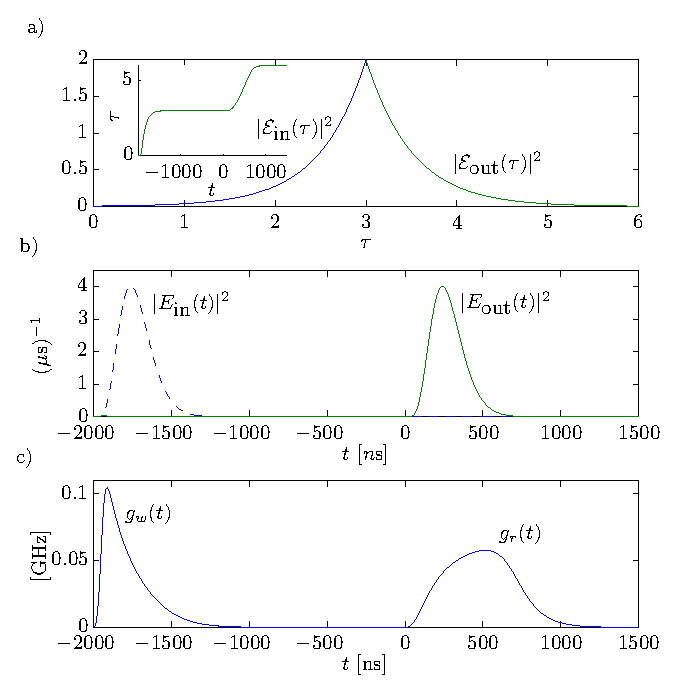
\epsfig{file=figure2v2.eps,width=\columnwidth,height=2.in}
\caption{Optimal memory performance is achieved when the effective input and output fields ${\cal E}_{in}(\tau)$ and ${\cal E}_{out}(\tau)$ of Eq. (\ref{eff-fields}) are related by a reversal of the effective time $\tau$ of Eq. (\ref{tau}) (a). This does not restrict the time dependence of the real fields $E_{in}(t)$ and $E_{out}(t)$ (b), provided the write and read couplings $g_w(t)$ and $g_r(t)$ are chosen appropriately (c). Any $E_{in}(t)$ can be absorbed with the optimal efficiency $\eta_w=1-e^{-2\tau_w}$ for $g_w(t)$ satisfying Eq. (\ref{couplings}); and $E_{out}(t)$ can, for example, be chosen to be proportional to $E_{in}(t-T)$ (where $T$ is the storage time) for $g_r(t)$ satisfying Eq. (\ref{couplings}).} \label{levels}
\end{figure}

This means in particular that memory performance can be optimal even if the input and output fields are not related by time reversal in real time. For example, let us suppose that we want the input and output fields to have the same temporal shape, $E_{out}(t)=\sqrt{\eta_w \eta_r} E_{in}(t-T)$, where $T$ is the storage time, while still satisfying Eq. (\ref{fieldst}). By inverting Eq. (\ref{fieldst}) one can show that this can be achieved by choosing the following time-dependent couplings for the write and read processes:
\begin{eqnarray}
g_w(t)=\sqrt{\frac{\kappa \eta_w |E_{in}(t)|^2}{2(1-\eta_w+\eta_w \int_{-\infty}^t dt'|E_{in}(t')|^2)}} \nonumber\\
g_r(t)=\sqrt{\frac{\kappa \eta_r |E_{in}(t-T)|^2}{2(1-\eta_r \int_{-\infty}^t dt'|E_{in}(t'-T)|^2)}} \label{couplings}.
\end{eqnarray}
This choice of $g_w(t)$ achieves the optimal write efficiency $\eta_w=1-e^{-2\tau_w}$ for any input field $E_{in}(t)$ and any value of $\tau_w=\int_{-\infty}^0 dt g_w^2(t)/\kappa$. On the other hand, the above choice of $g_r(t)$ ensures that the output field is exactly proportional to the input field (only displaced in time by $T$). We have seen that the read efficiency always satisfies
 $\eta_r=1-e^{-2\tau_r}$ with $\tau_r=\int_0^{\infty} dt g_r^2(t)/\kappa$.



{\it Spontaneous decay.} So far we have neglected the spontaneous decay rate $\gamma$. It is not difficult to include in the above approach. It does of course lead to somewhat lower efficiencies, because its effect is irreversible. The optimum input field can still be found by functional differentiation. To discuss the simplest example, let us consider square coupling pulses of strength $g_{w(r)}$ and duration $t_{w(r)}$. Then the optimized input field for writing is
\begin{eqnarray}
E_{in}(t) \propto g_w e^{\frac{g_w^2 t}{\kappa}+\gamma t}
\end{eqnarray}
and the output field from the read process is
\begin{eqnarray}
E_{out}(t) \propto g_r e^{-\frac{g_r^2 t}{\kappa}-\gamma t},
\end{eqnarray}
while the efficiencies satisfy
\begin{equation}
\eta_{w}=\frac{\frac{g_w^2}{\kappa}}{\frac{g_w^2}{\kappa}+\gamma}
\left(1-e^{-2(\frac{g_w^2}{\kappa}+\gamma) t_w} \right)
\end{equation}
{\bf Derive formula for read efficiency.} One can see that the relevant quantity is the ratio $C=\frac{g^2}{\kappa \gamma}$, which is essentially the optical depth in the presence of the cavity. High efficiencies require large $C$. For a given decay rate, $C$ can in principle always be increased by increasing $g$ (which requires increasing the dipole moment or the number of atoms), or by decreasing $\kappa$ (which requires increasing the finesse of the cavity, i.e. the number of roundtrips).

{\it Detuning.} There can also be a detuning $\Delta(t)$. Optimum input has a phase dependence that exactly compensates this detuning. If this is not possible, efficiencies will again be reduced. In analogy to the case of spontaneous decay, the effect will be small as long as the ratio $\frac{g^2}{\kappa \Delta}$ is large.

{\it Implementation.} In certain rare-earth doped crystals transitions can be switched on and off by changing the applied magnetic field. {\bf Not sure how generic the effect is. Learn a bit more about underlying theory.} Predictions most accurate when g tensors are known. First principles calculation from crystal field theory also possible. Two examples have been studied in detail, Tm:YAG and Nd:YVO ...
Magnetic switching. {\bf Not sure yet what to say exactly.} Fast switching of required field strengths is possible...

Have to make sure Zeeman splittings are always larger than pulse widths (is that even true?). Make sure time-dependent detuning is not too large...


{\it Discussion and Outlook.}

The described memory is attractive from a practical point of view as a solid-state Raman-type memory that does not require an optical control field, thus avoids optical noise. Discussed rare-earth doped crystals, other materials might work too, e.g. NV centers. Free-space theory is also possible, similar to free-space Raman, some things are known. Precise role of effective time etc. is work for future.

More conceptually, may also serve as a simple model protocol which may help to clarify the basic principles underlying various (all?) quantum memory protocols for light. In particular we have seen that the optimal write process is related to the read process, not (in general) by a reversal of the real time variable, but by a reversal of effective time. This is of course related to results of Kraus et al, Gorshkov et al. etc. The present model provides additional insight. Two strengths: first, in a sense simplest possible memory (switching of coupling is always necessary), second, emphasis on effective rather than real time clarifies precise role of time reversal. Open question: can all known protocols (including AFC etc.) be mapped onto this model? Can it serve as a kind of Rosetta stone?

(This is not to suggest that all protocols are equivalent, e.g. multimode properties are definitely different for AFC vs CRIB vs EIT/Raman. But maybe that could be part of the mapping etc. Fascinating questions for future...)




We thank ... for useful discussions. This work was supported by AITF, NSERC, China Scholarship Council ...

\begin{thebibliography}{99}
\bibitem{lvovsky} Lvovsky Nature Photonics
\bibitem{hammerer} Hammerer RMP
\bibitem{simonEPJD} Simon et al EPJD
\bibitem{sangouardRMP} Sangouard et al RMP
\bibitem{lukinRMP} Lukin RMP
\bibitem{gorshkovPRL} Gorshkov PRL
\bibitem{EITexp} EIT experiments
\bibitem{nunn} Nunn PRA
\bibitem{Ramanexp} Raman experiment(s)
\bibitem{tittel} Tittel photon echo memories
\bibitem{echoexp} echo experiments
\bibitem{Guillot-Noel} Guillot-Noel PRB
\bibitem{GenevaDipole} Geneva dipole switching
\bibitem{Tamarat} Tamarat NV centers
\bibitem{GorshkovCavity} Gorshkov PRA cavity
\bibitem{IMQM} Afzelius and Simon, IM memory
\bibitem{vuletic} Vuletic cavity memory
\bibitem{kalachev} Kalachev phase matching


\end{thebibliography}


\end{document} 
